\chapter{Background}
\label{ch:background}

This chapter covers the concepts needed to understand the rest of the thesis. We keep the presentation minimal: for each topic, we introduce only what is directly used by the PACE architecture (Chapter~\ref{ch:pace}), by the experiments (Chapters~\ref{ch:experimental},~\ref{ch:rq2},~\ref{ch:rq3}), or by the discussion of related work in this thesis.

The chapter is organised in nine sections. Section~\ref{sec:bg-ec-deep-learning} introduces emergent communication within deep learning, which is the field regarding the thesis. Section~\ref{sec:bg-mdl} presents the minimum description length principle from library learning, which PACE uses to propose candidate abstractions. Section~\ref{sec:bg-bandits} presents multi-armed bandits from reinforcement learning, which PACE uses to decide whether to actually use those abstractions in messages. Section~\ref{sec:bg-mccarthy-pace-thesis} traces the line from McCarthy et al.'s human architect-builder game~\cite{mccarthy_learning_2021} to PACE and to this thesis. Section~\ref{sec:bg-what-languages-look-like} reviews the properties of emergent languages. Section~\ref{sec:bg-input-distribution} discusses the role of the input distribution. Section~\ref{sec:bg-populations} examines variation across populations, and Section~\ref{sec:bg-cross-population} reviews communication between independently trained agents. Section~\ref{sec:bg-positioning} positions this thesis within the landscape and points to the specific gaps we address.

\section{Emergent Communication in Deep Learning}
\label{sec:bg-ec-deep-learning}

Emergent communication is the study of the shared communication system developed by artificial agents that collaborate via interaction on a task, instead of being trained to reproduce pre-existing languages~\cite{lazaridou_emergent_2020}. This uses two neural agents, a speaker and a listener, trained together on a communication task in which the speaker's messages need to carry enough information for the listener to complete some goal on its own~\cite{foerster_learning_2016}. The classic example is the signalling game of Lewis~\cite{lewis_convention_1969}, illustrated in Figure~\ref{fig:lewis-game}: two agents cooperate to solve a coordination task, but only one of them observes the relevant state of the world, and the two can interact only through discrete messages whose meanings are not fixed in advance.

\begin{figure}[H]
    \centering
    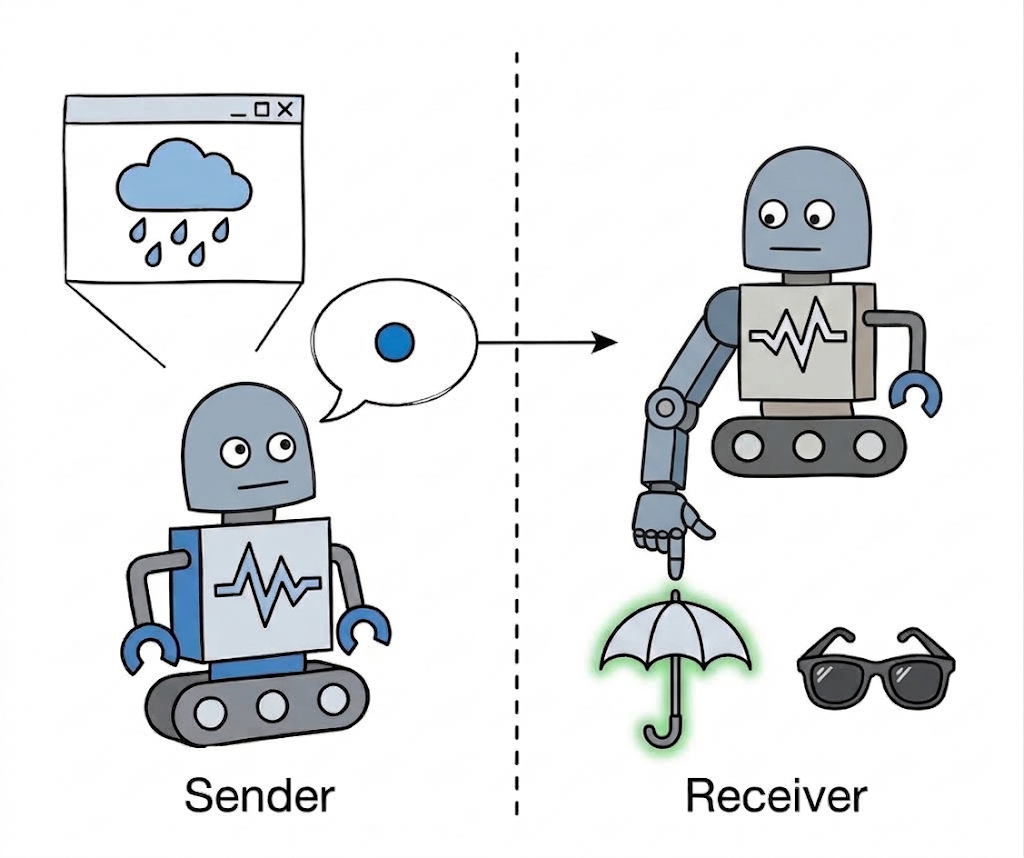
\includegraphics[width=0.68\textwidth]{images/figure_2_1_lewis_signalling_game.png}
    \caption{The classic Lewis signalling game~\cite{lewis_convention_1969}. The Sender observes the state of the world (in this example, rain) and produces a discrete message. The Receiver cannot see the world directly, but receives the message and must choose an appropriate action (in this case, the umbrella). Success requires both agents to converge on a shared meaning for an initially arbitrary message through repeated interaction. Modern deep-learning setups instantiate variants of this pattern with neural agents and richer state and action spaces.}
    \label{fig:lewis-game}
\end{figure}

Modern deep learning approaches instantiate variants of this basic pattern with neural agents. Different variants of the task exist. In referential games~\cite{lazaridou_multi-agent_2016,havrylov_emergence_2017}, the listener sees a set of candidate scenes and must identify the one the speaker saw. In signalling games~\cite{lewis_convention_1969,skyrms_signals_2010}, the listener directly reconstructs the target from the message. PACE, described in Chapter~\ref{ch:pace}, uses a signalling-game variant in which the listener predicts the next state of the scene given the current state and the speaker's message. Different sub-communities use slightly different names for these two roles. In the PACE paper that we build on, they are called the architect and the builder respectively, following the architect-builder game introduced by McCarthy et al.~\cite{mccarthy_learning_2021}. We keep the more general ``speaker'' and ``listener'' terminology throughout this thesis for consistency with the wider emergent communication literature, but the two pairs of names refer to the same pair of agents. The system is optimised end to end on the reconstruction or classification loss, and communication emerges as a byproduct of solving the task.

For an introduction to neural networks, their learning mechanisms, and reinforcement learning, see Mehlig~\cite{mehlig_machine_2019}.

The neural agents in these setups are typically encoder-decoder networks. The speaker's encoder maps the target scene into a hidden representation, and a decoder head then produces a categorical distribution over a fixed vocabulary of tokens, from which the discrete message is sampled. Their parameters are learned by backpropagating the task error through the network, following the general training principle introduced by Rumelhart et al.~\cite{rumelhart_learning_1986}. Since the sampled message is discrete, however, the gradient from the listener's loss cannot flow through the sampling step directly. Two common workarounds are the straight-through Gumbel-softmax estimator~\cite{jang_categorical_2017}, which relaxes the categorical distribution into a continuous approximation during backpropagation while keeping the forward pass discrete, and the REINFORCE estimator~\cite{williams1992simple}, which treats message sampling as a policy and updates the speaker with a policy gradient. Both are widely used, and both come with tradeoffs in terms of bias and variance.

A central question in this line of work is what kind of language emerges. Early results showed that emergent languages can be surprisingly effective on the task they were trained for while looking very unlike a natural language~\cite{kottur_natural_2017,chaabouni_compositionality_2020}: agents can develop non-compositional codes that assign one arbitrary token per scene, or codes whose apparent structure does not survive perturbations to the task. This observation motivated a strand of research on what conditions push emergent languages toward more natural-looking properties, such as compositionality, systematic generalisation to unseen combinations, and reuse of shared units across contexts.
A useful theoretical background for this question is the efficient-communication view of language. Natural languages are shaped by pressures that balance informativeness against production and processing cost~\cite{gibson_how_2019}. One signature of this pressure is that frequency correlates with form: frequent words tend to be shorter~\cite{zipf_human_1949}, and word length is better predicted by contextual informativity than by frequency alone~\cite{piantadosi_word_2011}. Speakers also choose shorter alternatives more often in predictive contexts~\cite{mahowald_infoinformation_2013}. This coupling of frequency, predictability, and structure is precisely what a uniform training distribution removes, and what motivates asking whether related pressures re-emerge in PACE under skewed input.


Prior work has explored interventions at two levels~\cite{kim2021emergent,michel_revisiting_2022,rita_role_2022,chaabouni_emergent_2022,rita_language_2024}. Some change the task or the population of agents, for example by exposing agents to distributional shifts during training, rotating listeners so that the speaker cannot overfit to a single partner, adding pressure on message length~\cite{rita_lazimpa_2020}, or introducing asymmetries between agents during learning~\cite{van_eecke_language_2022}. Others change the agents themselves, typically by adding an inductive bias toward reusable structure. For example, explicit pressures for positive signalling and positive listening can alleviate the joint-exploration problem and make learned communication more reliable in multi-agent reinforcement learning~\cite{eccles_biases_2019}. PACE, the architecture we build on, likewise introduces a structural bias, but does so by augmenting the neural agents with a symbolic component that periodically proposes new reusable sub-programs and decides whether to adopt them. In this respect it fits the broader neuro-symbolic programming perspective, in which gradient-trained neural modules are combined with explicit symbolic primitives and program structure~\cite{chaudhuri_neurosymbolic_2021}.

The most important gap in the current literature, for our purposes, concerns the role of the input distribution. Most emergent communication work trains agents on uniform samples over the input space: every scene appears with equal frequency, or with mild variations that do not systematically vary in shape. Natural linguistic input is very different: word frequencies in large corpora follow Zipfian distributions~\cite{zipf_human_1949}, in which a small number of items account for most of the occurrences; frequent words also tend to be shorter and more irregular~\cite{pinker_words_1999,bybee_frequency_2007,wu_morphological_2019}. Skew can affect learning as well as the forms eventually produced: artificial-language experiments show that Zipfian input can facilitate word segmentation in context because high-frequency items provide stable anchors for processing new sequences~\cite{kurumada_zipfian_2013}. Recent work has begun to examine related effects in emergent communication. Sevestre and Dupoux~\cite{sevestre_frequency_2025} train referential-game agents on Zipfian input using the same parametrisation we adopt here, $p(k) \propto k^{-\alpha}$, with $\alpha \to 0$ corresponding to a uniform distribution and larger $\alpha$ concentrating mass on the highest-ranked objects. They find that messages for frequent objects develop less compositional structure than messages for rare objects, echoing the irregular-verbs pattern of natural language. Their analysis, however, studies a purely neural referential game through topographic similarity, the standard aggregate compositionality metric for such settings~\cite{brighton_understanding_2006}. How input concentration shapes an inspectable symbolic vocabulary, its size, its reuse, and its transferability across populations remains open. That is the gap this thesis targets.

\section{Library Learning and the Minimum Description Length Principle}
\label{sec:bg-mdl}

Minimum description length (MDL) is a general principle for model selection~\cite{rissanen_modeling_1978,li_introduction_2008}. It says that the best model of some data is the one that lets us describe the data with the shortest total length, counting both the length of the model itself and the length of the data given the model. A model that overfits pays a high cost in its own description length; a model that underfits pays a high cost in the data description length. MDL formalises the tradeoff between the two.
Scoring rules inspired by MDL provide a local, symbolic instance of the informativeness-complexity tradeoff argued to shape human lexicons more broadly~\cite{gibson_how_2019,kemp_kinship_2012,zaslavsky_efficient_2018,macwhinney_word_2015}. Work on recursive numeral systems further shows that this tradeoff can involve the size of the stored lexicon and the average morphosyntactic complexity of the expressions constructed from it~\cite{denic_recursive_2024}, a close analogue of the choice between adding a reusable abstraction and retaining longer primitive programs.

Library learning and program synthesis seek reusable sub-programs that allow a system to express its data more compactly~\cite{gulwani_program_2017,tian_learning_2020,ellis_dreamcoder_2021,bowers_top-down_2023}. In PACE, each training scene is described by a sequence of primitive actions (details in Chapter~\ref{ch:pace}). When the data are represented as sequences of primitive actions, a simple scoring rule inspired by MDL can rank candidate sub-sequences by the number of tokens that would be saved by replacing each occurrence with a single reusable token. For a candidate sub-sequence of length $\ell$ that appears $f$ times in the data, this score is

\begin{equation}
\text{score} = f \times (\ell - 1).
\end{equation}

The intuition is straightforward. A sub-sequence of length $\ell$ that we replace with a single token saves $\ell - 1$ primitive action tokens per occurrence. Multiplying by the frequency $f$ gives the total number of tokens saved if the sub-sequence is adopted. The rule promotes sub-sequences that are simultaneously long and frequent, and demotes ones that are only long (rare, expensive to adopt) or only frequent (short, low return on adoption).

\section{Multi-Armed Bandits}
\label{sec:bg-bandits}

The multi-armed bandit is a stripped-down decision problem~\cite{sutton_reinforcement_1998,lattimore_bandit_2020}. On each step, the agent chooses one of a fixed set of actions (called arms), receives a scalar reward that depends stochastically on the chosen arm, and updates its estimate of that arm's value. The problem is stateless: the arms available on each step are the same, and the reward distribution associated with each arm does not depend on which arms were chosen before. The goal is to maximise cumulative reward over many steps.

The characteristic difficulty of the bandit problem is the exploration-exploitation dilemma. Exploiting means choosing the arm that currently looks best according to the agent's estimates, which is what maximises reward if the estimates are accurate. Exploring means choosing an arm that currently looks suboptimal, which is what improves the estimates and lets the agent discover better arms it may have underestimated. A pure exploiter never improves its knowledge and can get stuck on an arm that is far from optimal; a pure explorer never converges on the best arm.

Several strategies for balancing exploration and exploitation have been proposed, including upper confidence bound methods that add a term for uncertainty to the estimated value, and Thompson sampling that draws actions from a posterior over arm values~\cite{lattimore_bandit_2020,auer_finite-time_2002,thompson_likelihood_1933}. A simpler strategy is epsilon-greedy. Under epsilon-greedy, the agent picks the arm with the highest estimated value with probability $1 - \varepsilon$, and picks a uniformly random arm with probability $\varepsilon$. The parameter $\varepsilon$ controls how aggressively the agent explores. A low $\varepsilon$ produces mostly exploitation; a high $\varepsilon$ produces mostly exploration.

The estimated value of each arm is maintained by a running average of the rewards received when the arm was chosen. A simple incremental update rule is: after choosing arm $a$ and receiving reward $r$, the estimate $Q(a)$ is updated as

\begin{equation}
Q(a) \leftarrow Q(a) + \alpha \times (r - Q(a)),
\end{equation}

where $\alpha$ is a learning rate. The initial estimate $Q(a)$ can be set to a chosen constant for each arm.

This is essentially all we need. The bandit does not need to observe any state, nor to model transitions between states, and does not need to plan multiple steps ahead. How this bandit is used within PACE---that is, what the arms represent, how the reward is computed, and how the update loop is embedded into the training procedure---is discussed in detail in Chapter~\ref{ch:pace}.

\section{From McCarthy to PACE to This Thesis}
\label{sec:bg-mccarthy-pace-thesis}

The specific line of work this thesis extends starts from an experiment by McCarthy et al.~\cite{mccarthy_learning_2021} on how humans develop shared abstractions in their language when playing a collaborative task. In their setup, two human participants play a two-player communication game called the architect-builder game: a speaker, or architect, sees a target scene made of stacked blocks and must instruct a listener, or builder, who cannot see the target, on how to reconstruct it step by step. Over repeated interactions on the same scenes, McCarthy et al. observed a systematic behavioural shift. In the first trials, participants describe their scenes at the level of individual blocks (``place a horizontal red block''). Over time, they begin to introduce mid-level shortcuts referring to recurring substructures (``that's a tower''), and eventually to whole-scene shortcuts (``it looks like an H''). The lexicon they build up over the game is more abstract, shared between the two players and used to communicate shorter utterances, echoing earlier work on convention formation and repeated reference games~\cite{hawkins_convention-formation_2017,hawkins_characterizing_2020}.

McCarthy et al. designed a computational model of this linguistic behaviour as a Bayesian model in which each participant balances two pressures: informativeness for the partner, and the cost of introducing new terms into the shared lexicon~\cite{mccarthy_learning_2021,goodman_pragmatic_2016}. Varying the weight of the second pressure produces different trajectories of abstraction, with intermediate weights matching the human data most closely~\cite{mccarthy_learning_2021}.

A second finding of McCarthy et al. matters for this thesis in particular. Even as dyads converged on the same tower-level abstractions, the specific conventions they adopted for those towers diverged from one another: the pairwise Jensen-Shannon divergence between dyads' word-frequency distributions grew significantly over repeated interaction, with different dyads settling into distinct lexical clusters~\cite{mccarthy_learning_2021}. Shared structural pressure produced a shared backbone of abstractions, but the conventions built on top of it remained population-specific, matching broader evidence that conventions can be both community-level and partner-specific~\cite{hawkins_generalizing_2020}. This is the human precedent for the dialect question we take up in RQ2 (Chapter~\ref{ch:rq2}), where PACE populations trained on the same distribution shape but different rankings develop divergent abstraction libraries. The axis of divergence differs: McCarthy et al. observe it growing over interaction time at fixed stimuli, whereas we observe it growing with input concentration at fixed training. The phenomenon is the same: populations that share structure can still diverge in convention.

The conventions that dyads form in these games are also partner-specific: a label negotiated with one partner does not automatically transfer to a new one~\cite{ji_ad_2025,brennan_conceptual_1996}. Partners can nevertheless adapt rapidly when their initial lexical expectations differ, and their uncertainty about an association helps predict when such adaptation will be necessary~\cite{murthy_shades_2022}. This partner-specificity is the human counterpart of the cross-population mismatch we study in RQ3, where a vocabulary built by one PACE population is not readily interpretable by agents from another. Recent work also shows that ad hoc conventions can be sticky, persisting even as the referential context changes~\cite{ji_ad_2025}. Together, these results make the human convention literature directly relevant not only to the formation of local vocabularies in RQ2, but also to the transfer failures and adaptation dynamics studied in RQ3.

The setup has one important limitation as a study of how abstractions emerge in principle. Human participants come into the experiment with a lifetime of visual and linguistic experience. When they see a configuration of blocks that happens to resemble a letter or a familiar shape, they can lean on that prior experience to name it. It is difficult, from behavioural data alone, to separate what the two players actually construct during the game from what they already brought into the room. This is not a defect of the McCarthy et al. study; it is a general feature of experiments with human subjects on emergent communication.

PACE, developed by Thomas et al.~\cite{thomas_pace_2025} after related neural attempts to model the architect-builder setting~\cite{jergus2022multiagent}, addresses this by running the same architect-builder task with artificial agents in place of human participants. The two players are now neural networks that start with no prior visual or linguistic knowledge of the shapes they will encounter, and a symbolic component decides when to introduce new abstractions into their shared vocabulary. If these agents nonetheless develop shared abstractions over the course of training, the abstractions cannot be a residue of prior world knowledge, they must be a product of the communicative dynamic itself. PACE shows that this is indeed what happens: the architect's vocabulary grows over training, its programs become shorter, and the two agents remain able to communicate successfully throughout. The specific mechanism by which abstractions are proposed and adopted is different from McCarthy et al.'s Bayesian model, but the phenomenon it reproduces is the same.

This thesis extends the PACE setup in a specific direction, following the same conceptual arc: from human dyads that develop shared abstractions under prior bias, to bias-free agents that show the same phenomenon in a controlled setting, to bias-free agents facing more demanding distributional conditions. The specifics of what we ask are introduced in Chapter~\ref{ch:introduction} and developed in Chapters~\ref{ch:experimental},~\ref{ch:rq2}, and~\ref{ch:rq3}.

\section{What Emergent Languages Look Like}
\label{sec:bg-what-languages-look-like}

A first line of enquiry within emergent communication concerns the nature of the languages that agents actually develop. Early work established that emergent codes can be surprisingly effective at solving communication tasks while looking very different from natural language. Kottur et al.~\cite{kottur_natural_2017} showed that in a repeated question-answering task, two agents converge on an efficient code that essentially assigns one arbitrary token per scene, with no visible internal structure connecting these tokens to the scene properties they describe. The code succeeds on the task, but it does so without exhibiting any of the compositional structure that characterises human languages, where the meaning of a whole utterance derives systematically from the meanings of its parts. In contrast, Mordatch and Abbeel~\cite{mordatch_emergence_2017} demonstrated that grounded compositional communication can emerge in a multi-agent environment, with discrete symbols forming a vocabulary and syntax. Compositional signalling has also been examined in formal models beyond neural-agent settings~\cite{steinert-threlkeld_compositional_2016}.

Subsequent work made the diagnosis more precise. Bouchacourt and Baroni~\cite{bouchacourt_how_2018} found that successful communication can rely on visual representations that align closely across agents without capturing the conceptual properties of the depicted objects. Andreas~\cite{andreas_measuring_2019} developed a method for measuring compositionality by assessing how well learned representations can be approximated by composing inferred representational primitives. Chaabouni et al.~\cite{chaabouni_compositionality_2020} carried this line further, showing that compositionality does not spontaneously arise even under conditions that would favour it and that generalisation to novel scene combinations remains fragile. Ren et al.~\cite{ren_compositional_2020} showed that neural iterated learning can encourage more structured languages by amplifying their advantages in learnability, with benefits for generalisation. Moving beyond perception-oriented tasks, Guo et al.~\cite{guo_emergent_2023} introduced a reasoning game in which agents communicate high-level rules; the resulting languages support generalisation to unseen contextual attributes and transfer across contexts or tasks.

A parallel line of work has explored ways of endowing agents with richer language structures by combining neural methods with symbolic components. Jergéus et al.~\cite{jergus2022multiagent} developed a Deep Reinforcement Learning approach to procedural abstraction in an architect-builder-style task, though under a simplification of the game where the builder is assumed to immediately interpret abstractions the architect introduces. This assumption removes the very pressure that drives communicative efficiency, and it is one of the specific limitations that PACE addresses by keeping the builder's interpretation of new abstractions as a target of learning rather than a given.

Two features of this literature are directly relevant to the work in this thesis. First, most studies use quantitative metrics that summarise a language along one or two aggregate dimensions: adoption count, average message length, mutual information between messages and scene features. What these metrics rarely capture is the internal composition of the vocabulary itself, that is, what specific patterns from the training data end up encoded in the discrete tokens the agents adopt. PACE, with its explicit and inspectable abstraction tracker, makes this question directly answerable, and RQ2 of this thesis relies on precisely this property.

Second, the literature converges on the observation that what emerges depends heavily on the specific conditions of training: the task, the population, the amount of data, and the input distribution. This is important background for the empirical work in Chapters~\ref{ch:experimental} through~\ref{ch:rq3}, which asks how one particular condition -- the concentration of the input distribution -- shapes what emerges.

\section{Input Distribution in Emergent Communication}
\label{sec:bg-input-distribution}

A closely related line of work has looked at how properties of the training input shape the emergent language. This line is important background for RQ1 of this thesis and deserves separate treatment.

Rita et al.~\cite{rita_role_2022} conducted one of the most systematic studies of population effects on the language that emerges. Working with a referential game setup, they showed that agents in populations of different sizes develop languages that differ in average message length, in the level of ambiguity of their messages, and in how they trade off simplicity of encoding (fewer distinct tokens in the vocabulary) against expressivity (the ability to distinguish more concepts). Their work established that population size is not just a scaling parameter but shapes qualitative properties of the language, providing empirical grounding for the more general claim that training conditions determine emergent language structure.

At the interface of emergent communication and cognitive science, work by Denić and Szymanik~\cite{denic_recursive_2024} showed how the informativeness-complexity trade-off applies to recursive numeral systems: languages balance lexicon size and average morphosyntactic complexity, and can be positioned on a Pareto frontier (Figure~\ref{fig:pareto-frontier}) that describes this trade-off. The Pareto frontier is the set of configurations that cannot be improved on one dimension without a sacrifice on the other -- in this case, a language cannot become simpler (smaller lexicon) without also becoming less expressive (less able to distinguish concepts), and vice versa. Similar analyses in the study of human languages, such as Kemp and Regier~\cite{kemp_kinship_2012} on kinship categories and Zaslavsky et al.~\cite{zaslavsky_efficient_2018} on colour names, have established that natural languages tend to sit close to the Pareto-optimal region of this frontier -- a signature of pressures for efficient communication. What is far less understood is whether emergent languages in artificial agents show the same tendency, and under what training conditions they do or do not.

\begin{figure}[htbp]
    \centering
    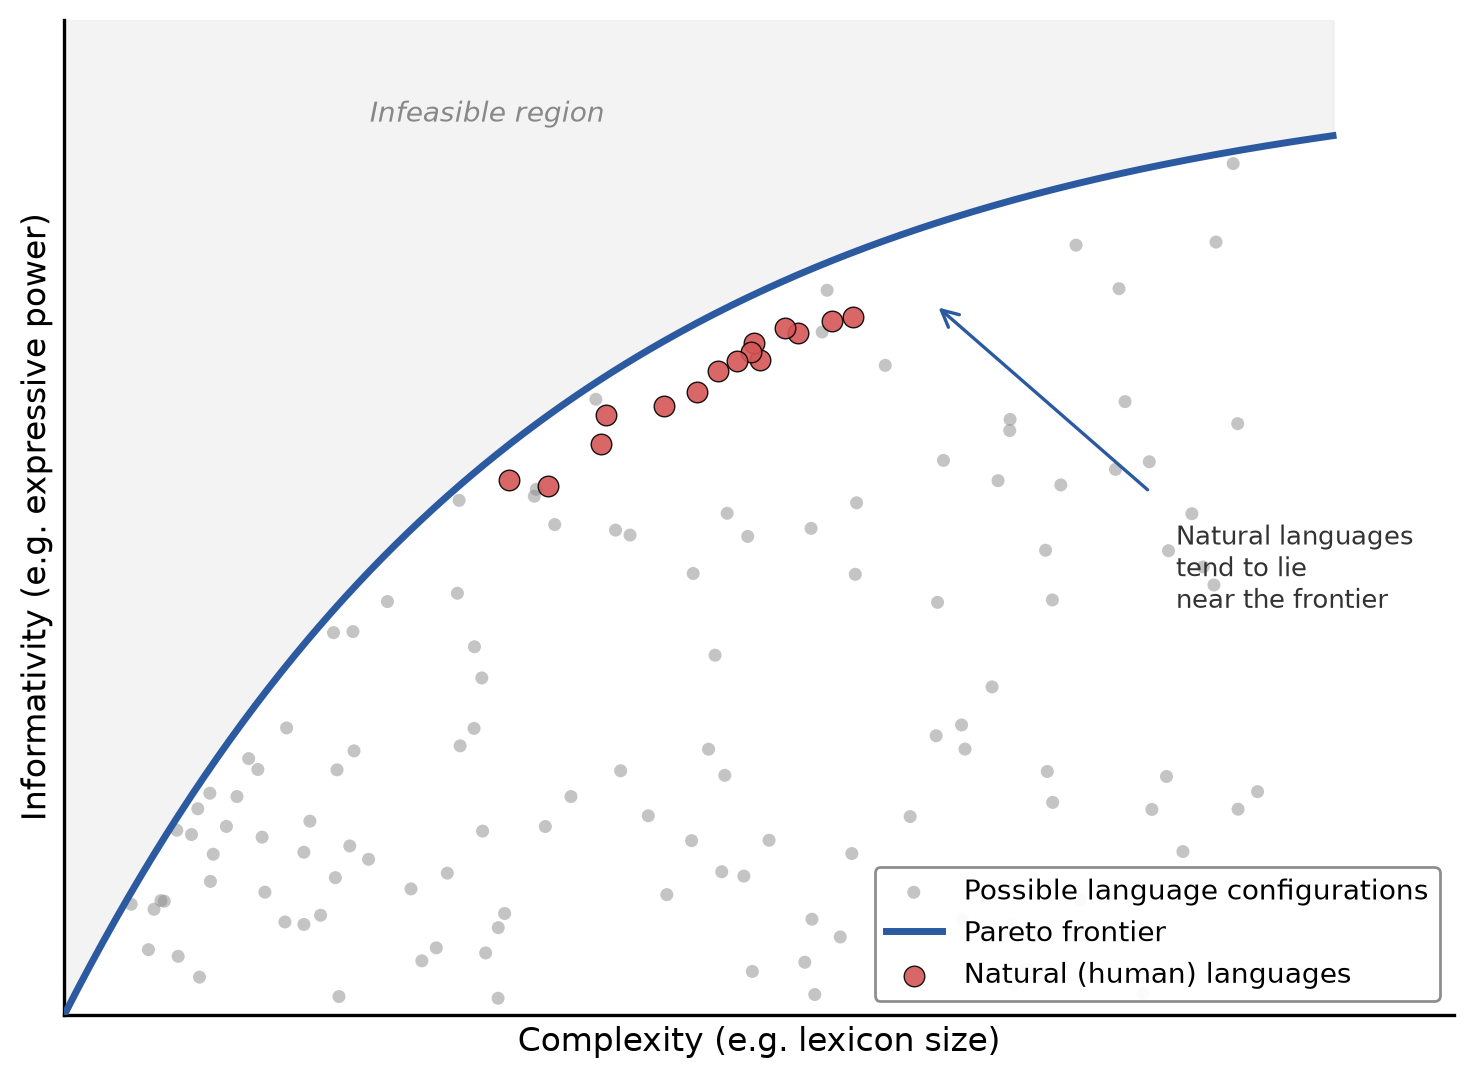
\includegraphics[width=0.75\textwidth]{images/pareto.png}
    \caption{Schematic illustration of the Pareto frontier for the informativity--complexity trade-off in language. Each grey dot represents a possible language configuration; the blue curve is the set of Pareto-optimal configurations, where informativity cannot be increased without also increasing complexity. Empirical work in cognitive science~\cite{kemp_kinship_2012,zaslavsky_efficient_2018,denic_recursive_2024} has shown that natural human languages tend to sit close to this frontier (red cluster), a signature of pressures for efficient communication.}
    \label{fig:pareto-frontier}
\end{figure}


The work of Steinert-Threlkeld and Szymanik~\cite{steinert-threlkeld_ease_2020} added an important computational-cognitive angle: they showed that languages closer to the Pareto frontier tend also to be easier to learn. This connects the Pareto question to the learning dynamics that PACE and similar systems implement: if pressures for efficient communication are met by more learnable languages, then the way an artificial agent learns and the language it converges to are not independent choices.

Systematic studies of how a controlled continuous parameter of the input distribution affects the emergent language remain rare in the deep-learning emergent communication literature. Most studies use a fixed distribution (typically uniform) and vary other factors, such as the task or the number of agents. This thesis explores this dimension directly: by parametrising the input distribution via a Zipfian concentration $\alpha$ and running the same PACE architecture across the full range, we isolate the effect of input concentration from other confounds.

\section{Populations and Cross-Agent Variation}
\label{sec:bg-populations}

A separate line of work has explored what happens when there are multiple pairs of communicating agents rather than just one. This literature is relevant background for RQ2 of this thesis, which asks how emergent vocabularies differ across independently trained populations of agents.

Early work by Havrylov and Titov~\cite{havrylov_emergence_2017} already noted that different runs of an emergent communication system, even with identical hyperparameters, produce languages that differ substantially in their surface form: different runs converge on different tokens for the same scene features, and there is no obvious mapping from one run's language to another. This is analogous to the classic observation from human language evolution that unrelated communities converge on very different labels for the same concepts.

More systematic study of population effects has emerged over recent years. Rita et al.~\cite{rita_role_2022} showed that when the same input distribution is presented to multiple independently trained pairs of agents, the resulting languages exhibit differences that are not just noise but reflect systematic variation shaped by the specific interactions each pair had. A distinct approach is neural iterated learning: Ren et al.~\cite{ren_compositional_2020} studied how transmitting a language across successive generations of agents can favour compositional structure. This intergenerational transmission differs from the independently trained populations compared in this thesis.

The question of \textit{why} independently trained agents converge on different languages, even from identical distributions, has been examined less thoroughly. One dimension is the random initialisation of the neural agents: different starting points lead to different exploration paths through the space of possible codes. Another dimension is the ordering of the data: the specific samples that the agents happen to see early in training can bias what they consolidate later. A third dimension, which this thesis explores, is the specific composition of the input distribution: even when two populations share the same distributional shape (that is, the same Zipfian concentration $\alpha$), the ranking permutation -- the specific assignment of scenes to the top positions of the frequency ranking -- can differ between populations. When two populations see the same distribution shape but with different scenes made most frequent, do they still converge on the same vocabulary?

The literature does not have a definitive answer to this question. Some work suggests that the answer depends on the strength of the compositional pressures: when strong pressures are present, populations converge more; when they are absent, populations diverge more. The specific setup of this thesis, with PACE's discrete vocabulary of adopted abstractions, allows the question to be posed at the level of the specific tokens two populations retain and share, which is a finer level of analysis than most previous work has attempted.

\section{Cross-Population Communication}
\label{sec:bg-cross-population}

The final line of related work concerns what happens when two agents that were trained separately are brought into contact. This is direct background for RQ3 of this thesis.

Within the broader multi-agent reinforcement learning literature (the study of how independent learning agents interact through shared environments and rewards), this question has been framed as \textit{zero-shot coordination}: the ability of an agent to succeed in a coordinated task with a partner it has never trained with. This should be distinguished from generalisation to unseen inputs. For example, the generalisation gains reported by Ren et al.~\cite{ren_compositional_2020} concern neural iterated learning and do not by themselves establish compatibility between independently learned codes. In a cross-population pairing, a potential obstacle is that the two agents may have assigned different meanings to the same symbols, even if each code works well within its original pair.

Work on this problem has focused on two directions. The first is enforcing structural properties on the emergent code that should transfer across pairs, such as compositionality~\cite{chaabouni_compositionality_2020,ren_compositional_2020}. If the code is compositional, the argument goes, an unfamiliar partner should be able to derive the meaning of composite messages from their parts, even without having seen those specific compositions during training. In practice, however, this argument has been tested less than it has been made, and the empirical evidence for it remains mixed. The second direction is population-based training: rather than train each agent with a single partner, agents can be trained by rotating through a pool of partners, encouraging them to develop codes that generalise across the pool. Some empirical evidence supports this, though the improvements tend to be modest.

Most existing work on cross-agent generalisation has been done in tasks where the two agents share exactly the same training distribution but differ only in random initialisation. What has been studied much less is the case where two agents come from \textit{different} distributions. This is a natural next question, given that natural communicative situations routinely involve speakers from different linguistic communities. In this thesis, RQ3 explores exactly this question, using cross-population pairings across a range of concentration parameters $\alpha$. The metrics we use to characterise adaptation difficulty (Section~\ref{sec:rq3-c-design}) are designed to distinguish among the alternative hypotheses that the previous literature has proposed for what should determine cross-agent success.

The picture that emerges from our experiments diverges in some respects from the naive expectations set by earlier work. This is discussed in detail in Chapter~\ref{ch:rq3}, but it is worth noting here that the tension between our findings and the existing literature is one of the substantive contributions of this thesis, and that Chapter~\ref{ch:rq3} devotes explicit space to reconciling the two.

\section{Positioning of This Work}
\label{sec:bg-positioning}

The thesis sits at the intersection of two of the lines described above, and more broadly within efficient-communication approaches to language structure~\cite{kemp_kinship_2012,zaslavsky_efficient_2018,gibson_how_2019}. On one side, it belongs to the strand of emergent communication research that studies how properties of the training setup shape the properties of the emergent language. On the other side, it uses an architecture (PACE) that has an explicit interpretable component we can inspect and manipulate, rather than a pure end-to-end neural agent whose language is only observable through aggregate metrics.

Within this positioning, the specific gap we target concerns the role of the input distribution. Most emergent communication work uses uniform training input. A systematic characterisation of how the concentration parameter of the input distribution affects the internal structure of the emergent language, the divergence between the languages of different populations, and the robustness of communication across populations is still missing. This thesis provides that characterisation for the PACE architecture.

The architectural control is described in detail in Section~\ref{sec:pace-extensions}. In short, the thesis changes the training distribution and adds cross-pairing evaluation, while leaving the neural agents, the bandit, and the MDL proposal mechanism unchanged.